\chapter{Results}
\label{chap:results}

This chapter reports what the protocol of Chapter~\ref{chap:method} measured. It is organised
around the experiments rather than around the research question, and the answer to RQ1 is
assembled only in Section~\ref{sec:selection}, from the selection rule that was fixed in writing
before any of these numbers existed.

Two properties of the protocol shape every section that follows. First, the separation of
surfaces held throughout: accuracy is hardware-independent under greedy decoding with a fixed
grammar and is measured on the workstation, while every latency, throughput and memory figure is
measured on the target Raspberry~Pi~5. Second, the split between reference-text input and audio
input is absolute here. Exp-1 reads the \emph{transcript} of each test item, not its audio, so
every accuracy figure in Sections~\ref{sec:exp1} to~\ref{sec:statistics} is an upper bound on what
the deployed pipeline achieves. Section~\ref{sec:exp0} measures the size of the gap that bound
conceals; closing it is Exp-3, which belongs to the \emph{M\'emoire d'Ing\'enieur} and has not run.

Every table in this chapter is rendered by \texttt{eval/tables.py} directly from the measurement
CSVs named in its caption. No figure in this chapter was transcribed by hand.

\section{Speaker sensitivity at the acoustic front end}
\label{sec:exp0}

The acoustic front end is a source of error that Exp-1 cannot see, and Exp-0 measures how large it
is before any language model is involved. Table~\ref{tab:asr-sensitivity} reports \acrfull{wer} for
\texttt{whisper.cpp tiny.en}~\cite{whispercpp} on 300 validated Common Voice English
clips~\cite{commonvoice}, bucketed by the accent metadata the corpus carries, alongside the
author's 200 recorded drone commands.

% Generated by eval/tables.py -- do not edit; edit the renderer and re-run.
\begin{table}[htbp]
  \centering
  \scriptsize
  \setlength{\tabcolsep}{3pt}
  \caption[Speech-recognition word error rate by accent bucket, unprompted decoder]{Word error rate of \texttt{whisper.cpp} \texttt{tiny.en}, unprompted decoder, on 300 validated Common Voice English clips in 15 accent buckets from the corpus's metadata, and on the author's recorded drone commands.}
  \label{tab:asr-sensitivity}
  \begin{tabular}{lrrrll}
    \toprule
    Accent bucket & n & words & WER \% & 95\% CI & S / D / I \\
    \midrule
    New Zealand English & 10 & 96 & 6.2 & [0.0, 16.3] & 3 / 1 / 2 \\
    Malaysian English & 3 & 29 & 13.8 & n too small & 3 / 1 / 0 \\
    Scottish English & 10 & 87 & 16.1 & [4.2, 29.7] & 13 / 0 / 1 \\
    Australian English & 22 & 175 & 16.6 & [7.7, 26.5] & 24 / 2 / 3 \\
    Other (free-text accent labels) & 3 & 24 & 16.7 & n too small & 4 / 0 / 0 \\
    England English & 45 & 444 & 17.6 & [11.1, 24.7] & 59 / 4 / 15 \\
    United States English & 57 & 504 & 17.9 & [12.0, 24.7] & 72 / 8 / 10 \\
    Canadian English & 24 & 209 & 19.1 & [8.3, 31.6] & 28 / 1 / 11 \\
    Welsh English & 6 & 43 & 23.3 & n too small & 6 / 1 / 3 \\
    Filipino & 6 & 50 & 24.0 & n too small & 8 / 1 / 3 \\
    Southern African (South Africa, Zimbabwe, Namibia) & 7 & 75 & 25.3 & n too small & 16 / 0 / 3 \\
    India and South Asia (India, Pakistan, Sri Lanka) & 80 & 721 & 27.9 & [22.5, 33.6] & 156 / 13 / 32 \\
    Irish English & 9 & 96 & 31.2 & n too small & 23 / 0 / 7 \\
    Singaporean English & 6 & 59 & 33.9 & n too small & 18 / 1 / 1 \\
    Hong Kong English & 12 & 105 & 49.5 & [35.0, 63.6] & 41 / 2 / 9 \\
    \textbf{Author (L2 English, domain commands)} & \textbf{200} & \textbf{1822} & \textbf{23.1} & \textbf{[20.3, 25.9]} & \textbf{282 / 71 / 68} \\
    \bottomrule
  \end{tabular}
  \par\medskip
  \begin{minipage}{\textwidth}\footnotesize\raggedright The author's WER is lower than 7 of the 15 accent buckets (53rd percentile of the bucket distribution). The comparison is indicative, not matched: the author read drone commands and the Common Voice speakers read general English, so the two figures are over different text. No pass/fail is claimed: the speaker-sensitivity requirement asks for a position, not a threshold. Domain prompt on Common Voice: 22.4\% $\to$ 22.9\% (+0.5 pp). Domain prompt on the author's commands: 23.1\% $\to$ 23.0\% ($-$0.1 pp). The deployed configuration keeps the prompt; this table positions the author without it, because only the unprompted pass puts both speakers under the same condition. Intervals are 95\% bootstrap intervals over utterances; a bucket under ten utterances reports \texttt{n too small}. S / D / I: substitutions, deletions and insertions. Source: \texttt{results/exp0.csv}.\end{minipage}
\end{table}


The author's \gls{wer} is 23.1\% with a 95\% confidence interval of [20.3, 25.9], which places the
author below 7 of the 15 accent buckets --- the 53rd percentile of the bucket distribution. NFR-11
asks for that position rather than for a threshold, and the position is unremarkable: the author is
neither an unusually easy nor an unusually hard speaker for this acoustic model. The spread across
buckets is the more consequential number. New~Zealand English is transcribed at 6.2\% and Hong Kong
English at 49.5\%, an eightfold range, and the largest bucket in the sample --- India and South
Asia, 80 utterances --- sits at 27.9\% [22.5, 33.6]. A system fielded against the operator
population this spread describes does not have one error rate.

Two cautions bound what Table~\ref{tab:asr-sensitivity} supports. The comparison is indicative
rather than matched: the author read drone commands and the Common Voice speakers read general
English, so the two figures are computed over different text, and no pass or fail is claimed from
their ordering. Nine of the fifteen buckets carry fewer than 15 utterances and their intervals are
reported as \texttt{n too small} rather than as numbers that would invite comparison they cannot
support.

The deployed configuration passes a domain prompt to the decoder; Table~\ref{tab:asr-sensitivity}
reports the unprompted pass, because only that condition puts both speakers under the same
treatment. The prompt's measured effect is small and its sign is not consistent: on Common Voice it
moves \gls{wer} from 22.4\% to 22.9\% (+0.5~pp), and on the author's commands from 23.1\% to 23.0\%
($-$0.1~pp). Neither movement exceeds the width of the confidence interval on either figure. The
prompt is retained because it is what the runtime ships, not because this experiment established a
benefit.

\paragraph{What this bounds.} A \gls{wer} in the low twenties is the input the language model would
receive in flight, and Exp-1 does not receive it. The exact-match figures that follow are therefore
ceilings. Quantifying the drop from ceiling to floor requires running the full pipeline on audio at
graded signal-to-noise ratios, which is Exp-3; the difference between exact match here and
\acrfull{crr} there is defined in Chapter~\ref{chap:method} precisely so that the \acrshort{stt}
cost can be read off as a single subtraction once that experiment exists.

\section{The multi-model benchmark}
\label{sec:exp1}

Table~\ref{tab:model-comparison} is the central measurement of this document: three fine-tuned
\acrfullpl{slm} at Q4\_K\_M and Q8\_0, decoded under the \acrfull{gbnf} constraint by
\texttt{llama.cpp}~\cite{llamacpp}, scored on three splits, with the Pi-side timing joined on.

% Generated by eval/tables.py -- do not edit; edit the renderer and re-run.
\begin{table}[htbp]
  \centering
  \scriptsize
  \setlength{\tabcolsep}{2pt}
  \caption[Model comparison on the deployed surface]{Each quantised artefact decoded by \texttt{llama.cpp} under the \acrshort{gbnf} grammar. Accuracy columns are fractions over 240 (\texttt{test\_synth}), 200 (\texttt{test\_golden}) and 150 (\texttt{test\_ood}) items, scored on the workstation; latency, throughput and memory were measured on the cooled Raspberry Pi 5, 60 trials per configuration.}
  \label{tab:model-comparison}
  \begin{tabular}{lllrrrrrlrl}
    \toprule
    Model & Quant & Split & Intent-F1 & Slot-F1 & \acrshort{em} & Safe-fail & Schema-valid & p50/p95 (ms) & tok/s & Mem. (GiB) \\
    \midrule
    Llama-3.2-1B & Q4\_K\_M & \texttt{test\_synth} & 0.991 & 0.975 & 0.958 & 0.000 & 1.000 & 1,351/2,282 & 14.53 & 1.63 \\
    Llama-3.2-1B & Q4\_K\_M & \texttt{test\_golden} & 0.996 & 0.945 & 0.910 & 0.000 & 1.000 & 1,351/2,282 & 14.53 & 1.63 \\
    Llama-3.2-1B & Q4\_K\_M & \texttt{test\_ood} & 0.897 & -- & 0.813 & 0.107 & 1.000 & 1,351/2,282 & 14.53 & 1.63 \\
    Llama-3.2-1B & Q8\_0 & \texttt{test\_synth} & 0.991 & 0.978 & 0.963 & 0.000 & 1.000 & -- & -- & -- \\
    Llama-3.2-1B & Q8\_0 & \texttt{test\_golden} & 0.996 & 0.948 & 0.915 & 0.000 & 1.000 & -- & -- & -- \\
    Llama-3.2-1B & Q8\_0 & \texttt{test\_ood} & 0.889 & -- & 0.800 & 0.100 & 1.000 & -- & -- & -- \\
    Qwen2.5-0.5B & Q4\_K\_M & \texttt{test\_synth} & 0.985 & 0.978 & 0.954 & 0.000 & 1.000 & 647/1,072 & 27.93 & 0.68 \\
    Qwen2.5-0.5B & Q4\_K\_M & \texttt{test\_golden} & 1.000 & 0.961 & 0.935 & 0.000 & 1.000 & 647/1,072 & 27.93 & 0.68 \\
    Qwen2.5-0.5B & Q4\_K\_M & \texttt{test\_ood} & 0.855 & -- & 0.747 & 0.158 & 1.000 & 647/1,072 & 27.93 & 0.68 \\
    Qwen2.5-0.5B & Q8\_0 & \texttt{test\_synth} & 0.990 & 0.978 & 0.958 & 0.000 & 1.000 & -- & -- & -- \\
    Qwen2.5-0.5B & Q8\_0 & \texttt{test\_golden} & 1.000 & 0.958 & 0.930 & 0.000 & 1.000 & -- & -- & -- \\
    Qwen2.5-0.5B & Q8\_0 & \texttt{test\_ood} & 0.846 & -- & 0.733 & 0.150 & 1.000 & -- & -- & -- \\
    SmolLM2-360M & Q4\_K\_M & \texttt{test\_synth} & 0.968 & 0.881 & 0.812 & 0.022 & 1.000 & 475/894 & 40.63 & 0.55 \\
    SmolLM2-360M & Q4\_K\_M & \texttt{test\_golden} & 0.954 & 0.848 & 0.760 & 0.042 & 1.000 & 475/894 & 40.63 & 0.55 \\
    SmolLM2-360M & Q4\_K\_M & \texttt{test\_ood} & 0.795 & -- & 0.660 & 0.059 & 1.000 & 475/894 & 40.63 & 0.55 \\
    SmolLM2-360M & Q8\_0 & \texttt{test\_synth} & 0.980 & 0.886 & 0.812 & 0.000 & 1.000 & -- & -- & -- \\
    SmolLM2-360M & Q8\_0 & \texttt{test\_golden} & 0.972 & 0.866 & 0.790 & 0.000 & 1.000 & -- & -- & -- \\
    SmolLM2-360M & Q8\_0 & \texttt{test\_ood} & 0.755 & -- & 0.607 & 0.068 & 1.000 & -- & -- & -- \\
    \bottomrule
  \end{tabular}
  \par\medskip
  \begin{minipage}{\textwidth}\footnotesize\raggedright Safe-fail is the share of errors that resolve to \texttt{unknown} or \texttt{hover}; p50/p95 is the language-model prefill and decode stages combined; Mem. is the peak resident set of the language-model process, in GiB. Only Q4\_K\_M was timed on the board, so a Q8\_0 row carries \texttt{--} there; Slot-F1 is \texttt{--} on \texttt{test\_ood}, whose 150 references carry no slots, and Table~\ref{tab:false-command} reports what the models emit there. Active cooler fitted, 0 of 180 scored trials throttled, 67.5--74.1 \textdegree{}C; the uncooled run is in Table~\ref{tab:thermal-headroom}. Sources: \texttt{results/surface\_b.csv} (accuracy) and \texttt{results/exp1\_cooled.csv} (timing).\end{minipage}
\end{table}


\paragraph{Accuracy.} On \texttt{test\_golden} --- real recorded speech through the real
\acrshort{stt} stack, and therefore the split of record --- Qwen2.5-0.5B~\cite{qwen25} reaches
0.935 exact match at Q4\_K\_M, Llama-3.2-1B~\cite{llama32} reaches 0.910, and
SmolLM2-360M~\cite{smollm2} reaches 0.760. The ordering does not follow parameter count: the
1.24~B model is beaten by the 0.49~B model by 2.5~pp, a result Section~\ref{sec:iso-parameter}
separates into its two contributing effects. Intent macro-F1 is above 95 for every configuration
and reaches 100.0 for Qwen2.5-0.5B on the golden split, so the errors that remain are
predominantly parameter errors inside a correctly identified intent rather than misidentified
commands.

\paragraph{Schema validity is 1.0000 everywhere, and that is by construction.} Every one of the
eighteen rows reports 100.0\% schema validity. Under the grammar this is not a measurement of the
model but a property of the decoder, and the only experiment in which the figure is free to move is
the ablation of Section~\ref{sec:grammar-ablation}. It is reported here because NFR-6 requires it
to be reported, not because the models earned it.

\paragraph{Slot-F1 is withheld on the abstention split.} Every \texttt{test\_ood} row carries
\texttt{--} rather than a number in the slot column. That split's 150 references are
\texttt{\{"intent":"unknown"\}} and carry no slots at all, so the metric has no dynamic range on
it: with zero gold slot pairs, precision is zero whenever the model emits any slot and the score
can only take one of two degenerate values. What the models do emit there is reported properly by
the false-command rate below.

\paragraph{Thermal state, and why two runs exist.} Exp-1 was executed twice. The first execution
predates the active cooler that the hardware specification declares, and it throttled on all 180
scored trials at a 1.5~GHz cap against the 2.4~GHz the \texttt{performance} governor pins. That
run measured a configuration this project never declared, so it is not the run of record; it is
retained and reported in Table~\ref{tab:thermal-headroom}, because NFR-10 requires the throttle
proportion always to be reported and because the difference between the two runs is itself a
measurement.

% Generated by eval/tables.py -- do not edit; edit the renderer and re-run.
\begin{table}[htbp]
  \centering
  \scriptsize
  \setlength{\tabcolsep}{3pt}
  \caption[Thermal headroom: cooled and uncooled benchmark runs]{The multi-model benchmark's run of record (\texttt{results/exp1\_cooled.csv}, active cooler fitted) against an earlier run without active cooling (\texttt{results/exp1.csv}). The protocol is otherwise identical: same board, same three Q4\_K\_M artefacts, 60 scored trials per configuration after a ten-minute warm-up, cores 1--3 pinned, \texttt{performance} governor, swap disabled. Accuracy is not repeated: it is scored on the workstation and does not depend on the board's clock.}
  \label{tab:thermal-headroom}
  \begin{tabular}{lllrrrr}
    \toprule
    Config & Run & Throttled trials & Max temp. (\textdegree{}C) & Decode p95 (ms) & \acrshort{slm} total p95 (ms) & tok/s \\
    \midrule
    Llama-3.2-1B Q4\_K\_M & cooled & 0\% & 70.8 & 1842.5 & 2282.4 & 14.53 \\
    Llama-3.2-1B Q4\_K\_M & uncooled & 100\% & 90.6 & 2458.8 & 3238.6 & 10.75 \\
    Qwen2.5-0.5B Q4\_K\_M & cooled & 0\% & 74.1 & 1033.2 & 1072.4 & 27.93 \\
    Qwen2.5-0.5B Q4\_K\_M & uncooled & 100\% & 90.6 & 1518.9 & 1771.5 & 18.13 \\
    SmolLM2-360M Q4\_K\_M & cooled & 0\% & 74.1 & 785.5 & 894.2 & 40.63 \\
    SmolLM2-360M Q4\_K\_M & uncooled & 100\% & 91.1 & 1338.9 & 1610.2 & 24.11 \\
    \bottomrule
  \end{tabular}
  \par\medskip
  \begin{minipage}{\textwidth}\footnotesize\raggedright \textbf{Throttling} (share of trials with a non-zero throttle flag, budget 5\%): cooled, worst configuration 0\% (meets); uncooled, worst configuration 100\% (misses). \textbf{Cooled relative to uncooled}: Llama-3.2-1B Q4\_K\_M, decode p95 $-$25.1\% and throughput +35.2\%; Qwen2.5-0.5B Q4\_K\_M, decode p95 $-$32.0\% and throughput +54.1\%; SmolLM2-360M Q4\_K\_M, decode p95 $-$41.3\% and throughput +68.5\%. The uncooled run was capped at 1.5 GHz against the 2.4 GHz the \texttt{performance} governor sets, a clock ratio of at least 1.6$\times$; the clock actually held was not logged. The largest throughput gain, 1.69$\times$ on SmolLM2-360M, is accounted for by the clock alone only if the throttled clock fell below 1.42 GHz.\end{minipage}
\end{table}


NFR-10 moves from 100\% of trials throttled, against a 5\% budget, to 0\%. The cost of the missing
cooler was 25.1\% to 41.3\% of decode p95 and 35.2\% to 68.5\% of throughput, largest on the
smallest model --- decode at Q4\_K\_M on this board is compute-bound, so it scales with the core
clock, and the 1.6$\times$ clock ratio bounds the effect from above. The gains do not reach that
ratio, so the throttle is the dominant term in the difference but not the only one. For a
\acrfull{sbc} deployment the operational reading is direct: on this class of hardware the
enclosure is a term in the latency budget, and a throughput figure quoted without its thermal
state is not reproducible.

\paragraph{Latency, throughput and memory.} On the cooled run, Qwen2.5-0.5B at Q4\_K\_M decodes at
27.93~tok/s with a combined prefill-plus-decode p95 of 1{,}072~ms, SmolLM2-360M at 40.63~tok/s and
894~ms, and Llama-3.2-1B at 14.53~tok/s and 2{,}282~ms. Against Table~6's decode allowance of
1{,}100~ms p95, Qwen2.5-0.5B (1{,}033~ms) and SmolLM2-360M (785~ms) meet the budget and
Llama-3.2-1B (1{,}842~ms) misses it by 67\%. Peak resident set size is 0.55~GB, 0.68~GB and
1.63~GB respectively, so NFR-9a's 2.5~GB ceiling is met by every configuration with the nearest
approach still 35\% clear.

The prefill allowance of 250~ms p95 is the one stage budget the selected configuration misses, and
the shape of the miss matters more than its size. Qwen2.5-0.5B posts a prefill p50 of 38.5~ms and a
p95 of 328.8~ms; only 8 of its 60 trials exceed the budget at all. That distribution is the
prompt-cache behaviour the protocol deliberately enables: the system-prompt prefix is resident
across requests, most calls pay a few tens of milliseconds, and a minority miss the cache and pay a
full prefill. Llama-3.2-1B's miss is of a different kind --- a p50 of 267.7~ms already exceeds the
budget, and 34 of 60 trials do. The distinction is between a tail and a level, and only the latter
is a property of the model. The combined \acrshort{slm} stage budget that both figures roll up
into, 1{,}350~ms, is met by Qwen2.5-0.5B with 278~ms to spare.

\paragraph{Abstention is missed by every configuration measured.} Two requirements fail here and
must be stated in the same breath as the accuracy figures they sit beside. NFR-9, the safe-failure
rate, has a budget of $\geq$~0.70 and measures between 0.0000 and 0.1579, pooling to 0.0530 over
528 errors. NFR-18, the false-command rate on out-of-distribution input, has a budget of
$\leq$~0.05 and measures between 0.1867 and 0.3933. Neither is a near miss: NFR-9 is missed by
roughly a factor of thirteen on the pooled figure and NFR-18 by a factor of four to eight, and no
configuration satisfies either. The two are one failure seen from two sides --- the system can emit
a well-formed command and can be stopped by its validator, but it has no mechanism for declining.
Per the escalation rule fixed in the project specification, both are re-baselined against the
measured figures and the re-baselining is recorded rather than the budgets being quietly adjusted;
a re-baselined constraint is not a satisfied one, and neither requirement is reported as met
anywhere in this document. The failure mode, its root cause and what would be required to address
it are analysed in the discussion of limitations that follows.

\section{Isolating model family from model size}
\label{sec:iso-parameter}

Section~\ref{sec:exp1} established that parameter count does not order the results. Two effects
are confounded in that observation, and Table~\ref{tab:iso-parameter} separates them by adding a
fourth model, H2O-Danube3-500M~\cite{danube3}, chosen for the control it provides rather than as a
deployment candidate: at 514~M parameters it sits within 4.0\% of Qwen2.5-0.5B's 494~M, so the
pair differs in family while holding size approximately fixed.

% Generated by eval/tables.py -- do not edit; edit the renderer and re-run.
\begin{table}[htbp]
  \centering
  \footnotesize
  \setlength{\tabcolsep}{5pt}
  \caption{FP16 under \texttt{transformers}, fine-tuned, greedy. Generated by \texttt{eval/tables.py} from \texttt{train/kaggle\_out/surface\_a.csv}; parameter counts and families from \texttt{train/configs/*.yaml}. Ordered by parameter count.}
  \label{tab:iso-parameter}
  \begin{tabular}{lrlrrr}
    \toprule
    Model & Params & Family & test\_synth & test\_golden & test\_ood \\
    \midrule
    \texttt{smollm2-360m-instruct} & 362 M & HuggingFace (SmolLM2) & 0.8250 & 0.7750 & 0.6200 \\
    \texttt{qwen2.5-0.5b-instruct} & 494 M & Alibaba (Qwen2.5) & 0.9542 & 0.9350 & 0.7267 \\
    \texttt{h2o-danube3-500m-chat} & 514 M & H2O.ai (Danube3) & 0.8875 & 0.8700 & 0.7200 \\
    \texttt{llama-3.2-1b-instruct} & 1,236 M & Meta (Llama-3.2) & 0.9583 & 0.9250 & 0.7333 \\
    \bottomrule
  \end{tabular}
  \par\medskip
  \begin{minipage}{\textwidth}\footnotesize \#\#\#\# The two effects, separated - \textbf{Family, at matched size} (\texttt{qwen2.5-0.5b-instruct} 494 M vs \texttt{h2o-danube3-500m-chat} 514 M --- 4.0\% apart): \textbf{6.5 pp} on \texttt{test\_golden} (0.9350 vs 0.8700). - \textbf{Size, across the full range} (\texttt{smollm2-360m-instruct} 362 M vs \texttt{llama-3.2-1b-instruct} 1,236 M, 3.4x): \textbf{+15.0 pp} on \texttt{test\_golden} (0.7750 -> 0.9250). - \textbf{The largest model is not the best.} \texttt{llama-3.2-1b-instruct} (1,236 M, 0.9250) is beaten on \texttt{test\_golden} by \texttt{qwen2.5-0.5b-instruct}. Parameter count does not order this table. Caveat carried from \texttt{train/configs/h2o-danube3-500m.yaml}: the recipe is frozen at three epochs for every model, and the per-epoch validation curves show \texttt{h2o-danube3-500m-chat} and \texttt{smollm2-360m-instruct} still improving at epoch 3 while the other two have converged. Part of any gap is therefore convergence under a fixed budget rather than capability. The claim this table supports is about performance \textbf{under an identical three-epoch budget}, not about capability.\end{minipage}
\end{table}


At matched size the family effect on \texttt{test\_golden} is 6.5~pp, with Qwen2.5-0.5B at 0.9350
against H2O-Danube3-500M at 0.8700. Across the full 3.4$\times$ span of the range the size effect
is 15.0~pp, from SmolLM2-360M at 0.7750 to Llama-3.2-1B at 0.9250. Family therefore accounts for
something on the order of two-fifths of what the full size range buys, measured on the same task
under the same recipe --- and the ordering is not monotone in parameters, since the largest model
in the table is beaten by a model with 40\% of its parameters. For a deployment selecting under a
memory and latency ceiling, this is the operationally useful finding in the accuracy results: at
the sub-billion scale the choice of pretrained family is a first-order decision rather than a
detail to be settled after the size is fixed.

One caveat constrains the claim and is carried on the table itself. The training recipe is frozen
at three epochs for every model, and the per-epoch validation curves show H2O-Danube3-500M and
SmolLM2-360M still improving at epoch 3 while Qwen2.5-0.5B and Llama-3.2-1B have converged. Part
of both gaps is therefore convergence under a fixed budget rather than capability. The claim the
table supports is about performance under an identical three-epoch budget, which is the condition
a practitioner with a fixed fine-tuning allowance actually faces, and it is not a claim about the
ceiling any of these families could reach.

\section{The quantisation delta}
\label{sec:quantisation-delta}

Table~\ref{tab:quantisation-delta} reports contribution C3: the accuracy difference between the
FP16 model on the workstation and the quantised \acrfull{gguf} artefact decoded under the grammar,
on the golden split.

% Generated by eval/tables.py -- do not edit; edit the renderer and re-run.
\begin{table}[htbp]
  \centering
  \footnotesize
  \setlength{\tabcolsep}{5pt}
  \caption{Surface A is FP16 under \texttt{transformers} with no grammar. Surface B is the same adapter merged, converted and quantised, decoded by \texttt{llama.cpp} under the GBNF constraint. The delta therefore measures the \emph{deployment pipeline}, not weight precision alone --- the grammar is part of what changes, and on out-of-domain input it is the dominant term.}
  \label{tab:quantisation-delta}
  \begin{tabular}{llrrr}
    \toprule
    Model & Quant & FP16 EM (surface A) & Quantised EM (surface B) & Delta (pp) \\
    \midrule
    llama-3.2-1b-instruct & Q4\_K\_M & 92.5 & 91.0 & -1.5 \\
    llama-3.2-1b-instruct & Q8\_0 & 92.5 & 91.5 & -1.0 \\
    qwen2.5-0.5b-instruct & Q4\_K\_M & 93.5 & 93.5 & +0.0 \\
    qwen2.5-0.5b-instruct & Q8\_0 & 93.5 & 93.0 & -0.5 \\
    smollm2-360m-instruct & Q4\_K\_M & 77.5 & 76.0 & -1.5 \\
    smollm2-360m-instruct & Q8\_0 & 77.5 & 79.0 & +1.5 \\
    \bottomrule
  \end{tabular}
\end{table}


The deltas span $-$1.5~pp to $+$1.5~pp. Llama-3.2-1B loses 1.5~pp at Q4\_K\_M and 1.0~pp at Q8\_0;
Qwen2.5-0.5B loses nothing at Q4\_K\_M and 0.5~pp at Q8\_0; SmolLM2-360M loses 1.5~pp at Q4\_K\_M
and \emph{gains} 1.5~pp at Q8\_0. A quantised model scoring above its own FP16 parent is the
clearest available evidence about the scale of these numbers: at $n = 200$ a 1.5~pp difference is
three items, and no mechanism by which 8-bit weights improve on 16-bit ones is proposed here. The
whole column is consistent with measurement noise, and Section~\ref{sec:statistics} tests that
reading directly rather than leaving it as an impression.

What this delta does \emph{not} isolate is weight precision, and the table's own caption says so.
Three things change between the two surfaces at once --- the numeric format, the inference runtime,
and the presence of the decoding grammar --- so the difference measures the deployment pipeline as
a whole. This is the quantity a practitioner deciding whether to ship a quantised artefact needs,
and it is deliberately not the quantity a study of quantisation error would report. The
literature measuring quantisation degradation on downstream tasks at larger
scales~\cite{kurtic2025,kurt2026} reports the isolated effect; the number here is a different and
coarser one, and the two should not be read against each other. One of the three confounded terms
is separable with the data already collected --- decoding the quantised artefact a second time with
the grammar disabled holds precision and runtime fixed --- which is the ablation the next section
reports.

\section{The grammar ablation}
\label{sec:grammar-ablation}

Table~\ref{tab:grammar-ablation} removes the \gls{gbnf} constraint and changes nothing else: same
six artefacts, same 590 items, same greedy decode.

% Generated by eval/tables.py -- do not edit; edit the renderer and re-run.
\begin{table}[htbp]
  \centering
  \scriptsize
  \setlength{\tabcolsep}{3pt}
  \caption{Same six artefacts, same 590 items, same greedy decode; the only change is whether \texttt{llama.cpp} is given \texttt{schema/cmd.gbnf}. Decode p95 is \texttt{results/exp1.csv}, the Pi --- the workstation's decode time is not the deployed latency. It is pooled over the \textbf{three Q4\_K\_M configs only} (Exp-1 did not run Q8\_0 on hardware); the grammar-off row has no Pi measurement at all -- the ablation itself only ran on the workstation.}
  \label{tab:grammar-ablation}
  \begin{tabular}{lrrrrl}
    \toprule
    Condition & Items & Schema validity & Malformed & EM (pooled) & Decode p95 \\
    \midrule
    Grammar on & 3540 & 1.0000 & 0 & 0.8508 & 2110.4 ms \\
    Grammar off & 3540 & 0.9997 & 1 & 0.8492 & -- \\
    \bottomrule
  \end{tabular}
  \par\medskip
  \begin{minipage}{\textwidth}\footnotesize Pooled over every model, quantisation and split. Exact match is pooled by item, not averaged over the eighteen rows, so the larger splits carry their real weight.\end{minipage}
\end{table}


Pooled over 3{,}540 decodes, schema validity falls from 1.0000 to 0.9997 and exactly one output is
malformed. Exact match moves from 0.8508 to 0.8492, a difference of 0.16~pp. On this test set,
under these models, the grammar's measurable contribution to output validity is one command in
three and a half thousand.

That result confirms rather than undermines the argument for constrained decoding made in
Chapter~\ref{chap:related-work}, but only if it is read as the right kind of claim. The guarantee a
grammar provides is a statement about reachability --- no token sequence violating the schema is
reachable under the constraint, for any input whatsoever --- and a guarantee of that form is not
measured by a rate on a test set drawn from the same distribution as the training data. Three
epochs of supervised fine-tuning on a corpus of valid commands taught these models the output
format thoroughly enough that they rarely depart from it unprompted. A rate near zero is what a
successful fine-tune predicts; it says nothing about the input the fine-tune did not anticipate,
which is exactly the input a flight controller must be protected against. The one malformed output
is the entire measurable contribution on this distribution, and the guarantee is what covers the
distribution that was not sampled.

The cost side of the constraint is correspondingly small here. The literature reports that
grammar-constrained decoding can distort the output distribution~\cite{park2024} and degrade
reasoning performance on tasks requiring intermediate steps~\cite{tam2024}. Neither effect is
visible at this scale of task: 0.16~pp of exact match, in the direction that favours the grammar,
on a schema with ten intents and a bounded slot vocabulary. A single-turn classification-and-slot-
filling task under a small grammar is close to the best case for constrained decoding, and this
result should not be generalised past it.

There is a second reading of the same number, and it connects to the abstention failure recorded in
Section~\ref{sec:exp1}. The training that made the grammar nearly redundant is the training that
removed the model's willingness to decline: both are consequences of a corpus in which a
well-formed command is always the correct answer. The structural reliability and the absent
abstention are the same property observed twice.

\section{Statistical analysis}
\label{sec:statistics}

Exact match figures separated by two or three items invite over-reading, and the paired structure
of the data supports a direct test. Every configuration decodes the same items deterministically,
so predictions are paired per item and McNemar's test applies. Two confirmatory families were
declared: three pairwise model comparisons at Q4\_K\_M on the golden split, and three
quantisation comparisons within each model on the same split. Bonferroni correction within each
family of three gives $\alpha = 0.0167$ against a family-wise $\alpha = 0.05$. The exact binomial
test is used below 25 discordant pairs, where the chi-square approximation is not trustworthy, and
the continuity-corrected chi-square above it; both p-values are carried in
\texttt{results/mcnemar.csv} and the verdict agrees under either test for every row.

\paragraph{Model against model.} Qwen2.5-0.5B and Llama-3.2-1B are not separated: the two disagree
on 5 items out of 200, splitting them 5--0 in Qwen's favour, for an exact $p = 0.0625$ against
$\alpha = 0.0167$. Both are separated from SmolLM2-360M decisively --- $p = 2.5 \times 10^{-6}$
against Llama-3.2-1B and $p = 1.1 \times 10^{-7}$ against Qwen2.5-0.5B, on 38 and 41 discordant
pairs respectively. The measured 2.5~pp gap between the two leading models is therefore not
established as real by this evidence, while the 17.5~pp gap to the smallest model is.

\paragraph{Quantisation against quantisation.} No quantisation comparison reaches significance in
either family, confirmatory or descriptive. On the golden split the Llama-3.2-1B and Qwen2.5-0.5B
pairs each disagree on a single item out of 200 and return $p = 1$; the SmolLM2-360M pair disagrees
on 22 and returns $p = 0.286$. Read with Section~\ref{sec:quantisation-delta}, the conclusion is
that the quantisation deltas in Table~\ref{tab:quantisation-delta} are not distinguishable from
noise on this evidence.

\paragraph{Two cautions about how these results may be quoted.} First, a non-significant McNemar
is not a finding of equivalence. Where the discordant count is 1, the smallest attainable exact
p-value is 1.0 --- the test cannot reject regardless of what is true. What such a row establishes
is that the two artefacts disagreed on one item in 200, which is a bound on their difference worth
quoting, and is a different claim from the assertion that no difference exists. Second, an
identical exact match is not an identical model. SmolLM2-360M scores 0.8125 at both quantisations
on \texttt{test\_synth}, and the pairing shows why that coincidence is not a result: the two
artefacts disagree on 24 items and happen to split them 12--12. Comparing summary figures alone
would have reported a difference of exactly zero where there are two dozen of them, which is the
case for reporting the paired counts and not only the p-value.

\section{The selection rule applied}
\label{sec:selection}

The selection rule was fixed in writing before any result existed: \emph{the deployed model is the
configuration with the highest exact match among those satisfying NFR-2 and NFR-9a, ties breaking
toward lower p95 latency}. Applying it requires the constraint set first and the ranking second.

\begin{figure}[htbp]
  \centering
  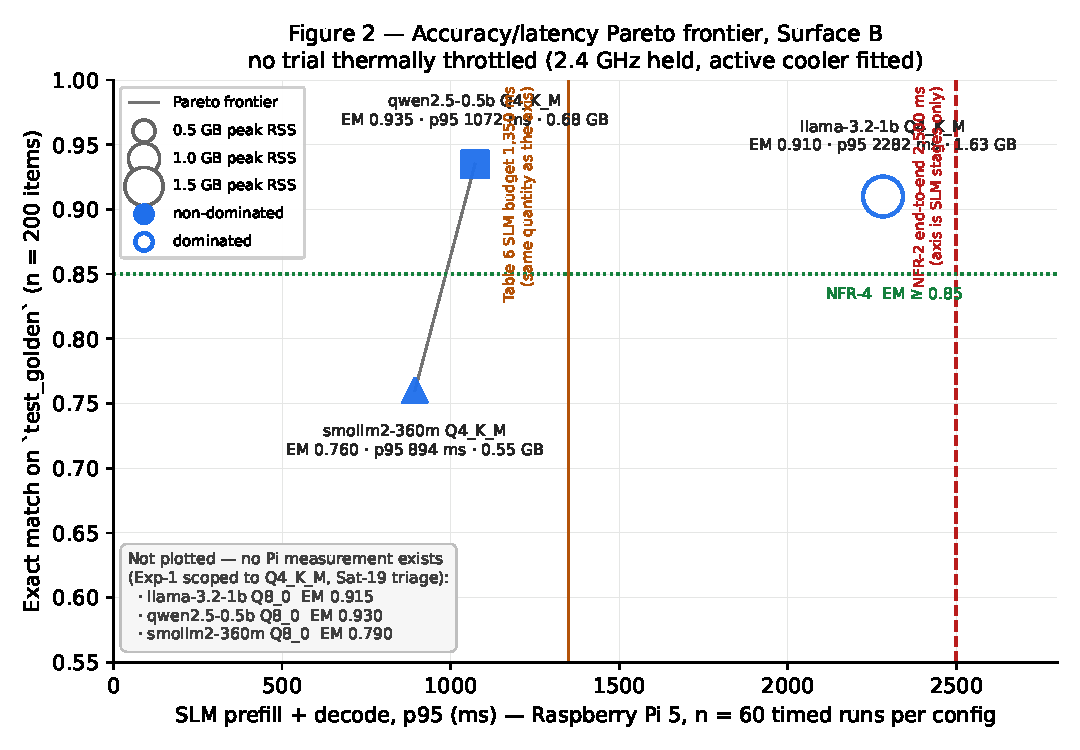
\includegraphics[width=\textwidth]{../results/figure2_pareto.pdf}
  \caption{Figure 2 --- the accuracy--latency Pareto frontier on Surface B, the quantised artefact
  under \texttt{llama.cpp} with the \gls{gbnf} constraint. Vertical axis is exact match on
  \texttt{test\_golden} ($n = 200$ items); horizontal axis is combined \acrshort{slm} prefill and
  decode p95 in milliseconds, measured on the cooled Raspberry~Pi~5 ($n = 60$ timed runs per
  configuration, no trial throttled). Marker area encodes peak resident set size. The solid
  vertical line is Table~6's \acrshort{slm} stage allowance of 1{,}350~ms, which is the same
  quantity as the axis; the dashed line at 2{,}500~ms is NFR-2, an end-to-end budget of which the
  axis measures only a part, so a point left of it has failed to rule itself out rather than passed.
  The horizontal line is NFR-4's exact-match floor of 0.85. Q8\_0 configurations are not plotted:
  Exp-1 was scoped to Q4\_K\_M on hardware, so no Pi latency exists for them. Generated by
  \texttt{eval/plots.py} from \texttt{results/surface\_b.csv} and
  \texttt{results/exp1\_cooled.csv}.}
  \label{fig:pareto}
\end{figure}

\paragraph{NFR-9a is satisfied by every configuration.} Peak resident set size is 0.55~GB, 0.68~GB
and 1.63~GB against a 2.5~GB ceiling. This constraint eliminates nothing.

\paragraph{NFR-2 has not been measured, and cannot be decided here.} NFR-2 bounds end-to-end
latency from end of speech at 2{,}500~ms p95. Exp-1 measures the \acrshort{slm} stages only, and
the remaining stages --- endpointing, \acrshort{stt}, validation and dispatch --- are Exp-2, which
belongs to the \emph{M\'emoire d'Ing\'enieur} and has not run. The constraint can therefore be
applied in one direction only. Because total latency is at least \acrshort{slm} latency on every
trial, the p95 of the total is at least the p95 of the \acrshort{slm} stages, and a configuration
whose \acrshort{slm} p95 already approaches 2{,}500~ms is ruled out without waiting for Exp-2.
Llama-3.2-1B's 2{,}282~ms leaves 218~ms for the rest of a pipeline whose \acrshort{stt} stage alone
is budgeted at 1{,}200~ms: it is eliminated. Qwen2.5-0.5B at 1{,}072~ms and SmolLM2-360M at 894~ms
are not eliminated by this argument, and neither is confirmed by it. This is the sense in which
Figure~\ref{fig:pareto}'s dashed line is drawn but not treated as a verdict.

\paragraph{The rule selects Qwen2.5-0.5B at Q4\_K\_M.} Among the configurations not eliminated,
exact match on the golden split is 0.935 for Qwen2.5-0.5B and 0.760 for SmolLM2-360M, and the rule
ranks on exact match without a tie to break. The selected configuration is also the only one of the
three meeting NFR-4's exact-match floor of 0.85, the 1{,}100~ms decode allowance, the 1{,}350~ms
combined stage allowance, the 20~tok/s throughput floor, NFR-9a and NFR-10 together. SmolLM2-360M
is faster on every timing measure and misses NFR-4 by 9~pp; Llama-3.2-1B is the largest model and
is beaten on accuracy by the model it is eliminated in favour of. Figure~\ref{fig:pareto} shows the
frontier this leaves: Qwen2.5-0.5B and SmolLM2-360M are non-dominated, and Llama-3.2-1B is
dominated on both axes simultaneously.

\paragraph{Three qualifications travel with this selection.} The margin over SmolLM2-360M is
established statistically; the margin over Llama-3.2-1B is not, and the choice between them rests
on the latency constraint rather than on the accuracy difference, which
Section~\ref{sec:statistics} declines to call real. The selection is made against reference-text
accuracy, and Section~\ref{sec:exp0} bounds how much of that accuracy the acoustic front end will
consume. And the selected configuration, like every other one measured, misses NFR-9 and NFR-18:
it is selected as the best available on the criteria the rule names, not as a configuration that
satisfies every requirement placed on the system. The discussion chapter takes up what that
costs and what it would take to fix. % \ref{chap:discussion} once ch5 exists
